% \begin{frame}
%     \frametitle{Дополнительные обозначения}
%     \begin{enumerate}
%         \item $D= \left( d_1, d_2, \dots, d_l \right)$, где $l$ - количество вершин, доступных для добавления.
%         \item $K$ - вектор длин критических путей от "головной" вершины до каждой вершины графа.
%         \item $\left( s_i, p_i \right)$ - достаточное количество информации для размещения работы в расписании. Установка соотношения между работой $t$ и парой $\left( s_i, p_i \right)$ и есть построение расписания
%     \end{enumerate}
%     \hrule
%     \vspace{2pt}
%     Жадные критерии
%     \begin{enumerate}
%         \item $GR1$ - критерий, используемый в выборе работы на постановку
%         \item $GR2$ - критерий, используемый в выборе места постановки работы
%     \end{enumerate}
%     \hrule
%     \vspace{2pt}
%     Процедуры ограниченного перебора
%     \begin{enumerate}
%         \item $H1$ - процедура перебора для создания места для постановки работы
%         \item $H2$ - процедура перебора для приближения времени старта работы к длине критического пути до нее
%     \end{enumerate}
% \end{frame}

\subsection{Схема}
\begin{frame}
    \frametitle{Общая схема алгоритма}
    {\tiny
        \ctikzfig{overview}
    }
\end{frame}

\subsection{Предподсчет}

\begin{frame}
    \frametitle{Жадный критерий выбора очередной работы}
    Из множества $\color{red}D$ выбирается работу по критерию $GC1$ максимальности количества потомков у вершины.
    \ctikzfig{max_children}
    Так же были проведены эксперименты с выбором максимальности количества предков.
    \vspace{1.3cm}
\end{frame}

\begin{frame}
    \frametitle{Различные критерии выбора очередной работы}
    \begin{figure}
        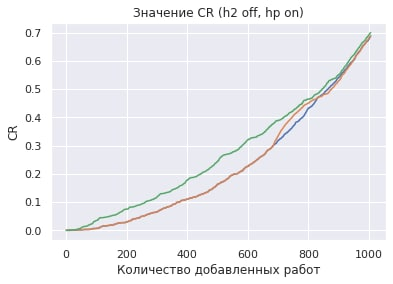
\includegraphics[width=8cm]{imgs/GC1_variants.jpg}
        \caption*{Изменение CR в различных критериях. Синий график - с выбором по количеству потомков, зеленый - по количеству предков, оранжевый - переключение критерия при достижения порогового значения}
    \end{figure}
\end{frame}

\begin{frame}
    \frametitle{Пробное размещение работы}
    Пробное размещение работы производится с учетом  жадного и дополнительных критериев. \\
    Жадный критерий $GC2$ - скорейшее завершение работы в расписании. \\
    Способы выбора места:
    \begin{enumerate}
        \item Подсчет усредненного взвешенного показателя среди критериев \\
              \begin{gather*}
                  crit_{CR} = C_1 \cdot GC2 + C_2 \cdot CR + C_3 \cdot CR2 \\
                  crit_{BF} = C_1 \cdot GC2 + C_2 \cdot BF
              \end{gather*}
              где $C_1$, $C_2$ и $C_3$ - параметры алгоритма. Работа размещается на место с наибольшим значением параметра $crit$.
        \item Допускные системы выбора
    \end{enumerate}
\end{frame}

\begin{frame}
    \frametitle{Допускная система выбора}
    \begin{enumerate}
        \item Список мест размещения работ ранжируется по $GC2$, после чего отсекаются верхние $n\%$ работ, где $n$ - параметр алгоритма
        \item Такие же действия повторяются для каждого дополнительного критерия
        \item В конечном списке выбрать место, лучшее \textbf{по времени} или \textbf{по дополнительному критерию}
    \end{enumerate}
    \begin{columns}
        \begin{column}{0.5\textwidth}
            \begin{center}
                С выбором по\\
                дополнительному критерию:\\
                BF: 3 \\
                Время выполнения расписания: 40584
            \end{center}
        \end{column}
        \begin{column}{0.5\textwidth}
            \begin{center}
                С выбором по времени: \\
                BF: 3 \\
                Время выполнения расписания: 5588
            \end{center}
        \end{column}
    \end{columns}
\end{frame}
